% Three ways to get to a star one unit away and back before a light pulse sent
% at departure reaches the star. Spacetime diagrams: distance x to the right,
% time t up, light at 45 degrees. Wedges are local light cones: the directions
% in which light can leave that event. A ship must always travel inside them.
%
% (a) Wormhole: mouths at x = 0.12 and 0.88 joined by a short throat. Ship at
%     speed 0.8 on the short legs; home at t = 0.60.
% (b) Warp drive: bubble at speed 3 each way. Inside the bubble the metric is
%     ds^2 = -dt^2 + (dx - v dt)^2, so light moves at dx/dt = v +- 1: the cone
%     edges have slopes 2 and 4 (outbound) and -2 and -4 (return). Home at 2/3.
% (c) Krasnikov tube: ds^2 = -(dt - dx)(dt + k dx), k = 1 outside and k = -1 + d
%     inside the tube (d = 0.15). Light moves along (1, 1) and along (-1, k):
%     inside, the second edge points down-left, (-1, -0.85). Outbound at speed
%     0.8 builds the tube (region t > x/0.8); the return follows (-1, -0.8),
%     inside the tipped cone, and arrives home at t = 1.25 - 0.8 = 0.45.
\documentclass[tikz,border=1pt]{standalone}
% Shared preamble for the standalone figures: the book's fonts, palette and
% drawing styles. Figures are drawn at their final printed size. A column is
% 3.35in (241pt) wide; a figure across both columns is 7in (505pt) wide.

\usepackage[T1]{fontenc}
\usepackage{newpxtext}
\usepackage[varbb]{newpxmath}
\usepackage[semibold,scale=0.95,lining]{sourcesanspro}
\usepackage{xcolor}
% Palette shared by the book and by the standalone figures in figures/src.
% One main hue (blue), one accent (orange), and a few roles used sparingly.

\definecolor{seblue}{HTML}{1D5B8F}    % headings, worked examples, main curves
\definecolor{seblueDark}{HTML}{123E63}
\definecolor{seorange}{HTML}{DC7A26}  % thought experiments, light and light cones
\definecolor{seteal}{HTML}{1F8577}    % checks, travellers and ships
\definecolor{sered}{HTML}{C0392B}     % negative energy, tension, violations
\definecolor{seviolet}{HTML}{5E548E}  % going deeper
\definecolor{sesand}{HTML}{8C6A3F}    % history
\definecolor{segray}{HTML}{6B7480}    % axes, guides, secondary labels
\definecolor{selight}{HTML}{D5DAE1}   % grids and faint rules

\usepackage{siunitx}
\usepackage{fontawesome5}
\usepackage{tikz}
\usetikzlibrary{arrows.meta,calc,positioning,decorations.pathreplacing,
  decorations.markings,shapes.geometric,fadings,shadings,patterns,3d,
  intersections,backgrounds}
\usepackage{pgfplots}
\pgfplotsset{compat=1.18}
\usepgfplotslibrary{fillbetween,groupplots,colormaps}

\tikzset{
  >={Latex[length=2.1mm,width=1.4mm]},
  every picture/.style={line cap=round, line join=round},
  lbl/.style={font=\sffamily\footnotesize, text=black!85},
  smalllbl/.style={font=\sffamily\scriptsize, text=black!75},
  guide/.style={segray, line width=0.4pt},
  axisline/.style={segray, line width=0.5pt, -{Latex[length=1.7mm,width=1.1mm]}},
  light/.style={seorange, line width=0.9pt},
  lightdash/.style={seorange, line width=0.9pt, dash pattern=on 3pt off 2pt},
  ship/.style={seteal, line width=1.4pt},
  cone/.style={fill=seorange!22, draw=seorange!85!black, line width=0.35pt},
}

\pgfplotsset{
  se axis/.style={
    axis lines=left,
    axis line style={segray, line width=0.5pt, -{Latex[length=1.6mm,width=1.1mm]}},
    tick style={segray, line width=0.4pt},
    major tick length=2.5pt,
    tick label style={font=\sffamily\scriptsize, text=black!75},
    label style={font=\sffamily\footnotesize, text=black!85},
    every axis plot/.append style={line width=1.1pt},
    legend style={font=\sffamily\scriptsize, draw=none, fill=none},
    scaled ticks=false,
    xticklabel={\sansnum{\tick}}, yticklabel={\sansnum{\tick}},
  },
}

% Numbers in figures are set in the sans-serif text font, with a true minus.
\sisetup{mode=text, reset-text-family=false, reset-text-series=false,
  reset-text-shape=false, drop-zero-decimal, group-minimum-digits=5}
% Tick values arrive as long decimals (1.5000000000); parse them first.
\newcommand{\sansnum}[1]{\begingroup\pgfkeys{/pgf/fpu=false}%
  \pgfmathparse{1*(#1)}\num{\pgfmathresult}\endgroup}

\begin{document}
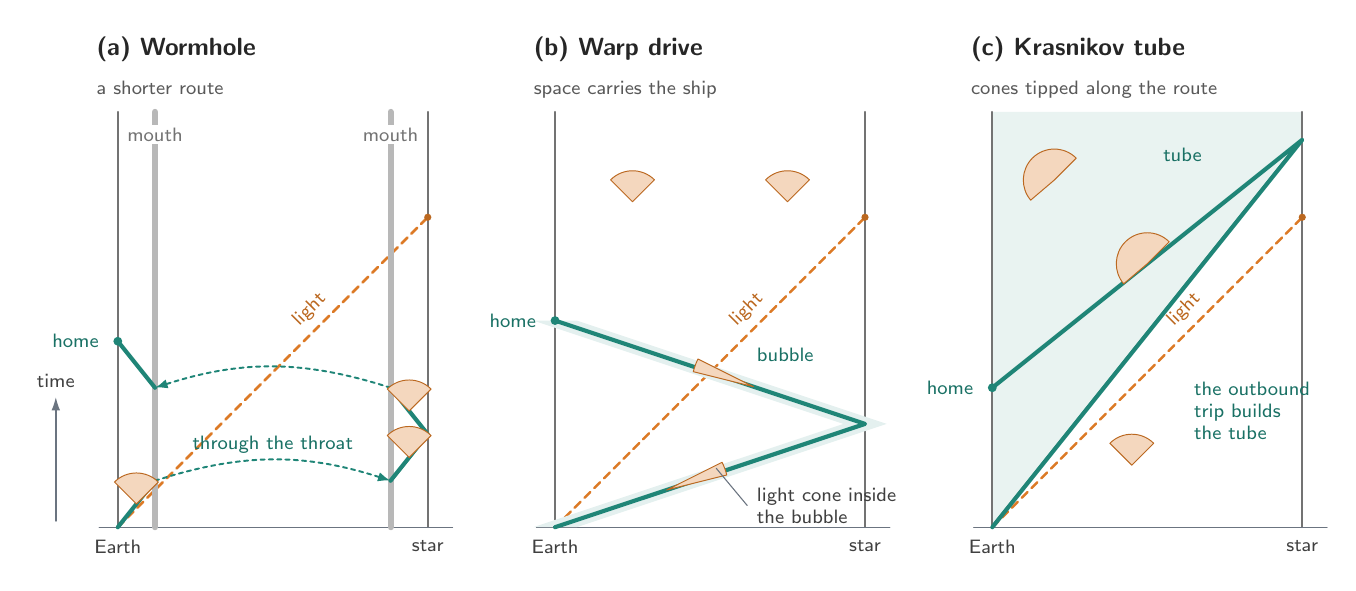
\begin{tikzpicture}[x=112pt, y=112pt,
  wl/.style={line width=0.7pt, black!55},
  pulse/.style={seorange, line width=0.9pt, dash pattern=on 3pt off 2pt},
  shippath/.style={seteal, line width=1.5pt},
  panel/.style={font=\sffamily\bfseries\small, text=black!85, anchor=south west},
  sub/.style={font=\sffamily\scriptsize, text=black!65, anchor=north west},
]
% a local light cone: #1 = apex, #2 and #3 = edge angles (counterclockwise from #2 to #3)
\newcommand{\cone}[4][0.1]{%
  \fill[seorange!30, draw=seorange!85!black, line width=0.35pt]
    #2 -- ++(#3:#1) arc[start angle=#3, end angle=#4, radius=#1] -- cycle;}
\newcommand{\panelframe}{%
  \draw[wl] (0,0) -- (0,1.34); \draw[wl] (1,0) -- (1,1.34);
  \draw[segray, line width=0.4pt] (-0.06,0) -- (1.08,0);
  \node[smalllbl, anchor=north] at (0,-0.01) {Earth};
  \node[smalllbl, anchor=north] at (1,-0.01) {star};
  \draw[pulse] (0,0) -- (1,1);
  \node[font=\sffamily\scriptsize, text=seorange!85!black, rotate=45, anchor=south]
    at (0.66,0.66) {light};
  \fill[seorange!85!black] (1,1) circle (1.3pt);}

% ------------------------------------------------------------------ (a)
\begin{scope}
\panelframe
\draw[black!28, line width=2.2pt] (0.12,0) -- (0.12,1.34);
\draw[black!28, line width=2.2pt] (0.88,0) -- (0.88,1.34);
\node[smalllbl, text=black!55, anchor=north, fill=white, inner sep=1pt] at (0.12,1.3) {mouth};
\node[smalllbl, text=black!55, anchor=north, fill=white, inner sep=1pt] at (0.88,1.3) {mouth};
\draw[shippath] (0,0) -- (0.12,0.15);
\draw[shippath] (0.88,0.15) -- (1,0.30) -- (0.88,0.45);
\draw[shippath] (0.12,0.45) -- (0,0.60);
\draw[seteal, line width=0.7pt, dash pattern=on 1.5pt off 1.5pt, -{Latex[length=1.6mm,width=1.2mm]}]
  (0.12,0.15) .. controls (0.4,0.24) and (0.6,0.24) .. (0.88,0.15);
\draw[seteal, line width=0.7pt, dash pattern=on 1.5pt off 1.5pt, -{Latex[length=1.6mm,width=1.2mm]}]
  (0.88,0.45) .. controls (0.6,0.54) and (0.4,0.54) .. (0.12,0.45);
\node[font=\sffamily\scriptsize, text=seteal!85!black] at (0.5,0.265) {through the throat};
\cone{(0.06,0.075)}{45}{135}
\cone{(0.94,0.225)}{45}{135}
\cone{(0.94,0.375)}{45}{135}
\fill[seteal] (0,0.60) circle (1.6pt);
\node[font=\sffamily\scriptsize, text=seteal!85!black, anchor=east] at (-0.03,0.60) {home};
\node[panel] at (-0.1,1.47) {(a) Wormhole};
\node[sub] at (-0.1,1.47) {a shorter route};
\end{scope}

% ------------------------------------------------------------------ (b)
\begin{scope}[xshift=158pt]
\panelframe
\fill[seteal!12] (-0.07,0) -- (0.07,0) -- (1.07,0.3333) -- (0.07,0.6667)
  -- (-0.07,0.6667) -- (0.93,0.3333) -- cycle;
\draw[shippath] (0,0) -- (1,0.3333) -- (0,0.6667);
\cone[0.2]{(0.36,0.12)}{14.04}{26.57}
\cone[0.2]{(0.64,0.4533)}{153.43}{165.96}
\cone{(0.25,1.05)}{45}{135}
\cone{(0.75,1.05)}{45}{135}
\draw[guide] (0.52,0.19) -- (0.62,0.07) node[smalllbl, anchor=west, align=left] {light cone inside\\the bubble};
\node[font=\sffamily\scriptsize, text=seteal!85!black, anchor=west] at (0.62,0.555) {bubble};
\fill[seteal] (0,0.6667) circle (1.6pt);
\node[font=\sffamily\scriptsize, text=seteal!85!black, anchor=east] at (-0.03,0.6667) {home};
\node[panel] at (-0.1,1.47) {(b) Warp drive};
\node[sub] at (-0.1,1.47) {space carries the ship};
\end{scope}

% ------------------------------------------------------------------ (c)
\begin{scope}[xshift=316pt]
\fill[seteal!10] (0,0) -- (1,1.25) -- (1,1.34) -- (0,1.34) -- cycle;
\panelframe
\draw[shippath] (0,0) -- (1,1.25) -- (0,0.45);
\cone{(0.45,0.2)}{45}{135}
\cone{(0.5,0.85)}{45}{220.36}
\cone{(0.2,1.12)}{45}{220.36}
\node[font=\sffamily\scriptsize, text=seteal!85!black, anchor=west, align=left]
  at (0.52,1.2) {tube};
\node[font=\sffamily\scriptsize, text=seteal!85!black, anchor=north west, align=left]
  at (0.62,0.5) {the outbound\\trip builds\\the tube};
\fill[seteal] (0,0.45) circle (1.6pt);
\node[font=\sffamily\scriptsize, text=seteal!85!black, anchor=east] at (-0.03,0.45) {home};
\node[panel] at (-0.1,1.47) {(c) Krasnikov tube};
\node[sub] at (-0.1,1.47) {cones tipped along the route};
\end{scope}

% time and distance, once
\draw[axisline] (-0.2,0.02) -- (-0.2,0.42) node[pos=1, anchor=south, smalllbl] {time};
\end{tikzpicture}
\end{document}
